% =====================================================================
% Note technique Nexialog — Critique méthodologique du GSE IRCANTEC
% Charte v2 (mai 2026). Polices Montserrat + Source Sans Pro avec repli
% automatique (Times + Helvetica) si non installées (réseau coupé).
% =====================================================================
\documentclass[11pt,a4paper]{article}

\usepackage[utf8]{inputenc}
\usepackage[T1]{fontenc}
\IfFileExists{sourcesanspro.sty}{\usepackage[default]{sourcesanspro}}{\usepackage{mathptmx}}
\IfFileExists{montserrat.sty}{\usepackage{montserrat}}{\usepackage[scaled=0.92]{helvet}}
\usepackage{microtype}
\usepackage{cmap}
\usepackage{geometry}
\usepackage{graphicx}
\usepackage{xcolor}
\usepackage{amsmath,amssymb,amsthm,mathtools,bm}
\usepackage{fancyhdr}
\usepackage{titlesec}
\usepackage[hyperref]{etoc}
\usepackage{enumitem}
\usepackage{tcolorbox}
\usepackage{xurl}
\usepackage{hyperref}
\usepackage{booktabs}
\usepackage{colortbl}
\usepackage{array}
\usepackage{longtable}
\usepackage{float}
\usepackage{caption}
\usepackage{pdflscape}
\usepackage{tabularx}
\usepackage{tikz}
\usetikzlibrary{arrows.meta,positioning,calc,fit,backgrounds}
\usepackage{needspace}
\usepackage{etoolbox}

\definecolor{nxnavy}{HTML}{002060}
\definecolor{nxred}{HTML}{B10031}
\definecolor{nxteal}{HTML}{409ABB}
\definecolor{nxslate}{HTML}{223E55}
\definecolor{nxgray}{HTML}{9A999E}
\definecolor{nxlightgray}{HTML}{D0D1D4}
\definecolor{nxoffwhite}{HTML}{F2F2F2}
\definecolor{nxgreen}{HTML}{2E7D32}
\definecolor{nxorange}{HTML}{F57C00}
\definecolor{nxlightblue}{HTML}{E6ECF7}

\geometry{a4paper, top=32mm, bottom=22mm, left=25mm, right=25mm,
          headheight=19mm, headsep=6mm}

\pagestyle{fancy}
\fancyhf{}
\fancyhead[L]{\parbox[c][14mm][c]{52mm}{\includegraphics[height=13mm]{logo_nexialog.pdf}}}
\fancyhead[R]{\parbox[c][14mm][c]{110mm}{\raggedleft\small Audit du GSE IRCANTEC~~\textbar~~\textit{Note critique méthodologique}}}
\fancyfoot[L]{\small Note critique --- Juin 2026}
\fancyfoot[R]{\small Page \thepage}
\renewcommand{\headrulewidth}{0pt}
\renewcommand{\footrulewidth}{0.3pt}
\renewcommand{\footrule}{\hbox to\headwidth{\color{nxlightgray}\leaders\hrule height \footrulewidth\hfill}}

\titleformat{\section}{\sffamily\Large\bfseries\color{nxnavy}}{\thesection.}{0.5em}{}
\titleformat{\subsection}{\sffamily\large\bfseries\color{nxnavy}}{}{0em}{\thesubsection.~}
\titleformat{\subsubsection}{\sffamily\normalsize\bfseries\color{nxnavy}}{}{0em}{\thesubsubsection.~}

\etocsetstyle{section}{}{}
  {\par\noindent\sffamily\large\bfseries\textcolor{nxred}{\etocname}\hfill\textcolor{nxred}{\etocpage}\par\medskip}{}
\etocsetstyle{subsection}{}{}
  {\par\noindent\hspace*{5mm}\sffamily\normalsize\mdseries\textcolor{nxnavy}{\etocname}\hfill\textcolor{nxnavy}{\etocpage}\par\vspace{6pt}}{}
\etocsetstyle{subsubsection}{}{}
  {\par\noindent\hspace*{10mm}\sffamily\small\mdseries\textcolor{nxnavy}{\etocname}\hfill\textcolor{nxnavy}{\etocpage}\par\vspace{5pt}}{}
\etocsettocstyle{}{}

\tcbuselibrary{skins,breakable}
\newtcolorbox{definitionbox}[1][]{enhanced, breakable,
  colback=nxlightblue, frame hidden, boxrule=0pt, arc=3pt,
  before skip=4mm, after skip=3mm, left=4mm, right=4mm, top=3mm, bottom=3mm}
\newtcolorbox{exemplebox}[1][Exemple]{enhanced, breakable,
  colback=nxoffwhite, frame hidden, boxrule=0pt, arc=3pt,
  fonttitle=\sffamily\bfseries\color{nxnavy}, title=#1,
  detach title, before upper={\tcbtitle\par\nobreak\medskip\nobreak},
  before skip=4mm, after skip=3mm, left=4mm, right=4mm, top=3mm, bottom=3mm}
\newtcolorbox{insightbox}[1][Point clé]{enhanced, breakable,
  colback=nxoffwhite, frame hidden, boxrule=0pt, arc=3pt,
  fonttitle=\sffamily\bfseries\color{nxred}, title=#1,
  detach title, before upper={\tcbtitle\par\nobreak\medskip\nobreak},
  before skip=4mm, after skip=3mm, left=4mm, right=4mm, top=3mm, bottom=3mm}
\newtcolorbox{mabox}[1][]{enhanced, breakable,
  colback=nxlightblue, frame hidden, boxrule=0pt, arc=3pt,
  fonttitle=\sffamily\bfseries\color{nxnavy}, title=#1,
  detach title, before upper={\tcbtitle\par\nobreak\medskip\nobreak},
  before skip=4mm, after skip=3mm, left=4mm, right=4mm, top=3mm, bottom=3mm}

\theoremstyle{definition}
\newtheorem{proposition}{Proposition}
\newtheorem{remarque}{Remarque}

\captionsetup{font=small,labelfont={bf,color=nxnavy},labelsep=period}
\setlength{\abovecaptionskip}{4pt}
\setlength{\belowcaptionskip}{4pt}
\setlength{\textfloatsep}{10pt plus 2pt minus 2pt}
\setlength{\floatsep}{8pt plus 2pt minus 2pt}
\setlength{\intextsep}{10pt plus 2pt minus 2pt}
\renewcommand{\topfraction}{0.92}
\renewcommand{\bottomfraction}{0.92}
\renewcommand{\textfraction}{0.05}
\renewcommand{\floatpagefraction}{0.85}
\widowpenalty=10000
\clubpenalty=10000

\setlist{leftmargin=*, labelindent=0pt, itemsep=2pt, topsep=4pt}

\pretocmd{\section}{\needspace{6\baselineskip}}{}{}
\pretocmd{\subsection}{\needspace{5\baselineskip}}{}{}
\pretocmd{\subsubsection}{\needspace{4\baselineskip}}{}{}
\BeforeBeginEnvironment{definitionbox}{\needspace{5\baselineskip}}
\BeforeBeginEnvironment{exemplebox}{\needspace{5\baselineskip}}
\BeforeBeginEnvironment{insightbox}{\needspace{5\baselineskip}}
\BeforeBeginEnvironment{mabox}{\needspace{4\baselineskip}}

\hypersetup{colorlinks=true, linkcolor=nxred, citecolor=nxred, urlcolor=nxred, linktoc=all}

\DeclareMathOperator{\Corr}{Corr}
\DeclareMathOperator{\Var}{Var}
\DeclareMathOperator{\Cov}{Cov}
\DeclareMathOperator{\Avar}{Avar}
\DeclareMathOperator{\diag}{diag}
\DeclareMathOperator{\tr}{tr}
\DeclareMathOperator*{\argmin}{arg\,min}
\DeclareMathOperator*{\argmax}{arg\,max}
\newcommand{\R}{\mathbb{R}}
\newcommand{\E}{\mathbb{E}}
\newcommand{\Prob}{\mathbb{P}}
\newcommand{\Ecal}{\mathcal{E}}
\newcommand{\Ncal}{\mathcal{N}}
\newcommand{\Xcal}{\mathcal{X}}
\newcommand{\Scal}{\mathcal{S}}
\newcommand{\Rcal}{\mathcal{R}}
\newcommand{\eps}{\varepsilon}
\newcommand{\transp}{^{\!\top}}

\setlength{\emergencystretch}{2.5em}
\tolerance=1200

\begin{document}

\begin{titlepage}
\thispagestyle{empty}
\vspace*{-5mm}
\begin{center}
  \includegraphics[width=0.55\textwidth]{logo_nexialog.pdf}
\end{center}
\vspace{1.6cm}
\begin{center}
  {\color{nxred}\rule{0.55\textwidth}{1.5pt}}\\[10mm]
  {\sffamily\bfseries\color{nxnavy}\fontsize{26pt}{32pt}\selectfont\MakeUppercase{Estimation et simulation}\\[4mm]\MakeUppercase{du GSE IRCANTEC}}\\[10mm]
  {\color{nxred}\rule{0.55\textwidth}{1.5pt}}\\[12mm]
  {\sffamily\normalsize\color{nxnavy}Juin 2026}
\end{center}
\vspace{12mm}
\noindent\begin{minipage}{\textwidth}\small
Cette note prolonge le diagnostic de la revue indépendante du générateur de scénarios économiques (GSE) monde-réel du régime IRCANTEC. Elle porte sur la robustesse de l'\emph{estimation} et de la \emph{simulation}, et propose un cadre unifié d'estimation jointe à régime latent commun. Trois fragilités méthodologiques sont analysées : (i)~le calibrage par cibles distributionnelles ; (ii)~le calibrage séparé du modèle à changement de régime et le calcul des corrélations par état ; (iii)~la simulation des régimes par variable uniforme commune.

\vspace{2mm}
Pour chaque point, la critique est étayée mathématiquement à partir des éléments documentés dans la revue, puis un correctif est spécifié : représentation autorégressive universelle, estimation par maximum de vraisemblance jointe --- avec \emph{formes fermées} explicites là où elles existent --- et simulation cohérente pilotée par une chaîne d'état unique. Document confidentiel, préparé à titre d'analyse méthodologique pour l'usage exclusif de l'IRCANTEC et de la Caisse des Dépôts.
\end{minipage}
\vfill
\begin{center}
  {\sffamily\bfseries\large\color{nxnavy}THINK SMART~~\textcolor{nxred}{$\bullet$}~~ACT DIFFERENT}
\end{center}
\end{titlepage}

\begingroup
\hypersetup{hidelinks}
\vspace*{\stretch{0.5}}
{\noindent\sffamily\Huge\bfseries\color{nxnavy}Table des matières\par}
\vspace{18mm}
\tableofcontents
\vspace*{\stretch{2}}
\endgroup
\newpage

\section{Objet et synthèse}

Le GSE du régime est techniquement soigné : schémas de discrétisation exacts là où ils existent, corrections de covariance sur la courbe nominale, régularisation semi-définie positive (SDP) des corrélations. La présente note ne remet pas en cause ces choix de \emph{modélisation} ; elle cible la \emph{méthode d'estimation} et le \emph{couplage} des facteurs, deux dimensions qui conditionnent directement la stabilité des sorties ALM d'un exercice à l'autre et la fidélité de la dépendance de queue. Trois points sont développés, puis un cadre unifié est proposé.

\begin{insightbox}[Les trois points critiques]
\textbf{(1) Calibrage par cibles distributionnelles.} L'appariement d'un petit nombre de moments stationnaires est un estimateur de minimum de distance, à forte variance et sensible à la fenêtre. Surtout, les cibles sont des quantités \emph{stationnaires} ($t\to\infty$) alors que la série historique est une trajectoire \emph{transitoire} courte, partant de conditions initiales figées hors régime stationnaire : les moyennes empiriques \emph{ne convergent pas} vers les cibles, et l'estimateur est biaisé.

\textbf{(2) Hardy séparé et corrélations par état.} La maximisation directe de vraisemblance est non robuste ; le calcul des corrélations stressées sur l'\emph{intersection} des fenêtres de stress propres à chaque facteur n'est pas viable (intersections vides, régime mal défini, perte de SDP) ; aucun facteur latent de marché commun n'est modélisé.

\textbf{(3) Simulation par uniforme commune.} Tirer l'état suivant de chaque chaîne à partir d'une même variable uniforme crée une dépendance \emph{comonotone} non estimée, dépendante de l'étiquetage, et incohérente avec l'hypothèse d'indépendance faite à l'estimation.
\end{insightbox}

\noindent\textbf{Proposition d'ensemble.} Tout facteur s'écrit, via sa discrétisation, comme une équation autorégressive dont les coefficients dépendent éventuellement du temps, de l'état et d'un processus de Markov d'état économique commun $\Ecal_t$. On calibre par \emph{maximum de vraisemblance jointe}, séquentiellement, en deux groupes (facteurs insensibles au régime, facteurs sensibles), avec corrélations estimées sur les résidus standardisés et \emph{formes fermées} explicites là où elles existent ; on simule directement à partir de cette représentation globale. La Table~\ref{tab:synth} résume le diagnostic et le correctif.

\section{Conventions et notations}

On fixe quelques conventions valables dans toute la note avant d'aborder les critiques.

Sauf mention contraire, $h=\Delta=1/12$ désigne le pas mensuel et $n\approx 240$ le nombre de points. Le \emph{processus de Markov d'état économique} est la chaîne $\Ecal_t\in\{1,\dots,K\}$, de matrice de transition $P=(p_{ab})$ et de loi invariante $\pi$ (la notation $\Ecal$ évite toute collision avec le pas $\Delta$). Le vecteur d'état du facteur $i$ est $Y^{(i)}_t\in\R^{d_i}$ ($d_i=2$ pour un Vasicek à deux facteurs, noté V2F, $d_i=1$ sinon). Les innovations standardisées sont $\eps_t$, de matrice de corrélation $\Omega(\Ecal_t)$ (éventuellement dépendante du régime). On note $f_i(\cdot\mid\cdot)$ la densité de transition conditionnelle exacte du facteur~$i$, $\Phi$ la fonction de répartition de $\Ncal(0,1)$, et $\Xcal_t$ l'information disponible en~$t$.

\section{Critique 1 --- le calibrage par cibles distributionnelles}

Cette section caractérise d'abord l'estimateur, puis établit trois fragilités : un mauvais conditionnement structurel, un biais de transitoire lié à l'initialisation hors régime stationnaire, et une perte d'efficience. Le correctif (vraisemblance conditionnelle exacte) est introduit en clôture et détaillé en Section~\ref{sec:cadre}.

\subsection{Nature de l'estimateur}

Le calibrage des V2F (inflation, taux réels) résout, en notant $m^{\mathrm{mod}}(\Theta_d)$ le vecteur des moments-modèle (volatilités, corrélations, écart-types stationnaires) et $m^{\mathrm{hist}}$ leurs analogues empiriques, le programme de minimum de distance suivant.

\begin{definitionbox}
\[
\hat\Theta_d=\argmin_{\Theta_d\in\R^4_+}\ \big(m^{\mathrm{mod}}(\Theta_d)-m^{\mathrm{hist}}\big)\transp\,W\,\big(m^{\mathrm{mod}}(\Theta_d)-m^{\mathrm{hist}}\big),
\qquad W=\diag(\lambda_v,\lambda_c,\lambda_s),
\]
où $\Theta_d=\{\kappa_1,\kappa_2,\sigma_1,\sigma_2\}$ et $(\lambda_v,\lambda_c,\lambda_s)$ pondèrent volatilité, corrélation et dispersion.
\end{definitionbox}

\noindent Il s'agit \emph{exactement} d'un estimateur GMM / minimum de distance à pondération \emph{diagonale imposée à dire d'expert}, et non à la pondération efficiente $W^\star=S^{-1}$ (inverse de la covariance de long terme des moments). Trois conséquences en découlent.

\subsection{Mauvais conditionnement et non-robustesse à la fenêtre}

La covariance asymptotique d'un estimateur de minimum de distance s'écrit
\[
\Avar(\hat\Theta_d)=\big(G\transp W G\big)^{-1}G\transp W\,S\,W G\big(G\transp W G\big)^{-1},
\qquad G=\frac{\partial m^{\mathrm{mod}}}{\partial\Theta_d\transp}.
\]
Dès que la jacobienne $G$ est mal conditionnée, $\Avar$ explose : une faible variation de $m^{\mathrm{hist}}$ (changement de fenêtre, ajout de données, changement de fréquence d'observation) induit une forte variation de $\hat\Theta_d$. Or ce mauvais conditionnement est \emph{structurel} pour les modèles à retour à la moyenne. Pour un facteur d'Ornstein--Uhlenbeck $dx=\kappa(\theta-x)\,dt+\sigma\,dW$, la variance stationnaire vaut $\Var_\infty(x)=\sigma^2/2\kappa$, de sorte que tout moment construit sur la \emph{dispersion stationnaire} n'identifie que le \emph{rapport} $\sigma^2/\kappa$, jamais $\sigma$ et $\kappa$ séparément. La séparation repose entièrement sur les moments de volatilité des \emph{variations} et l'autocorrélation, peu informatifs au pas mensuel sur des séries très persistantes : l'objectif est quasi plat le long de la crête $\sigma^2/\kappa=\text{cste}$.

\paragraph{Preuve empirique tirée de la revue.} L'instabilité n'est pas théorique. Sur les \emph{mêmes} données, le passage de la régression linéaire (estimateur exact, cf.\ \S\ref{sec:closed}) aux cibles distributionnelles déplace fortement les paramètres (Table~\ref{tab:instab}), et la simple bascule mensuel~$\to$~annuel de la régression fait passer le retour à la moyenne court des taux réels de $125{,}7\,\%$ à $310{,}2\,\%$ ($\times\,2{,}5$). Le point décisif est la \emph{direction systématique} : les cibles distributionnelles produisent un $\kappa$ plus faible et un $\sigma$ plus élevé --- exactement la signature du biais établi au~\S\ref{sec:transient}.

\begin{table}[h]
\centering\small
\renewcommand{\arraystretch}{1.25}
\begin{tabular}{@{}l c c c@{}}
\toprule
\textbf{Paramètre (facteur long terme)} & \textbf{Régression$^{\ast}$} & \textbf{Cibles distrib.} & \textbf{Direction} \\
\midrule
Inflation --- $\kappa_2$ (retour à la moyenne) & $69{,}8\,\%$ & $35{,}8\,\%$ & $\div\,1{,}95$ \\
Inflation --- $\sigma_2$ (volatilité) & $0{,}5\,\%$ & $1{,}3\,\%$ & $\times\,2{,}6$ \\
Taux réels --- $\kappa_2$ (retour à la moyenne) & $33{,}6\,\%$ & $10{,}8\,\%$ & $\div\,3{,}1$ \\
Taux réels --- $\sigma_2$ (volatilité) & $0{,}6\,\%$ & $0{,}9\,\%$ & $\times\,1{,}5$ \\
\bottomrule
\end{tabular}
\caption{Écart entre méthodes d'estimation \emph{sur les mêmes données} (source : tables inflation et taux réels de la revue). $^{\ast}$~régression linéaire sur données mensuelles. Les cibles distributionnelles abaissent systématiquement $\kappa$ et relèvent $\sigma$ : la dispersion de niveau visée est gonflée, et le modèle l'absorbe en élargissant $\sigma^2/2\kappa$.}
\label{tab:instab}
\end{table}

\subsection{Initialisation hors régime stationnaire et biais de transitoire}
\label{sec:transient}

C'est le point central, et il est \emph{interne} au modèle : il ne suppose à aucun moment de contester la spécification d'Ornstein--Uhlenbeck. Le V2F est ergodique : avec $\kappa_1,\kappa_2>0$ il admet une loi stationnaire gaussienne, et les cibles $\sigma^{\mathrm{mod}}_Y(\tau)$, $\sigma^{\mathrm{mod}}_{\Delta Y}(\tau)$, $\rho^{\mathrm{mod}}_{\Delta Y}$ sont, \emph{par construction}, des fonctionnelles de la \emph{distribution stationnaire} --- la revue le pose explicitement (« hypothèse de stationnarité », analyse \emph{restreinte à la distribution stationnaire}). Ces cibles sont donc des limites $t\to\infty$.

\paragraph{Le décalage.} Le processus n'est \emph{pas} initialisé dans son régime stationnaire. Les valeurs initiales $(r_0,m_0)$ (taux réels), $(q^s_0,q^l_0)$ (inflation) sont \emph{figées} : calées sur la courbe initiale et les scénarios du COR, donc \emph{pas} tirées de $\Ncal(\mu_\infty,\Sigma_\infty)$. Les propres formules de lien de la revue le portent d'ailleurs explicitement, via des termes transitoires du type $e^{-\alpha\Delta}(r_0-\mu)$. Posons l'état $X_t=(r_t,m_t)\transp$ suivant $dX=A(\mu_\infty-X)\,dt+\Sigma_w^{1/2}\,dW$, $A$ stable de valeurs propres $\kappa_1,\kappa_2>0$. La solution exacte depuis $X_0$ se décompose comme suit.

\begin{definitionbox}
\[
X_t=\underbrace{\mu_\infty}_{\text{niveau LT}}+\underbrace{e^{-At}\,(X_0-\mu_\infty)}_{\textstyle d_t\ :\ \text{transitoire déterministe}}+\underbrace{s_t}_{\text{partie stationnaire, } \Var\to\Sigma_\infty},
\qquad \Sigma_\infty:\ A\Sigma_\infty+\Sigma_\infty A\transp=\Sigma_w.
\]
\end{definitionbox}

\noindent La cible de dispersion vise $\sigma^{\mathrm{mod}}_Y=\sqrt{B\Sigma_\infty B\transp}$ ($B$ : sensibilités prix-taux). L'estimateur historique, lui, est calculé sur \emph{une} trajectoire issue de $X_0$ figé.

\paragraph{Non-convergence de la moyenne empirique.} La moyenne temporelle hérite du transitoire :
\[
\bar X=\mu_\infty+\frac1n\sum_{k} e^{-At_k}(X_0-\mu_\infty)+\frac1n\sum_k s_{t_k}
\ \approx\ \mu_\infty+\underbrace{\tfrac1T A^{-1}\!\big(I-e^{-AT}\big)(X_0-\mu_\infty)}_{=\,O(1/(\kappa T))\ \neq\ 0}+o_p(1).
\]
Le terme central \emph{ne s'annule pas} tant que $\kappa T=O(1)$ : $\bar X$ est un estimateur \emph{biaisé} de $\mu_\infty$. Et c'est précisément le régime dans lequel on se trouve --- les demi-vies impliquées par les $\kappa$ calibrés sont \emph{comparables à la fenêtre} (Table~\ref{tab:halflife}). Le théorème ergodique reste vrai asymptotiquement, mais sa vitesse est gouvernée par le temps de mélange $\sim 1/\kappa$ : en échantillon fini, la moyenne de trajectoire reflète la \emph{réalisation} (une décrue séculaire des taux) et non la moyenne d'ensemble.

\begin{table}[h]
\centering\small
\renewcommand{\arraystretch}{1.25}
\begin{tabular}{@{}l c c c@{}}
\toprule
\textbf{Facteur} & $\kappa$ \textbf{(cibles distrib.)} & \textbf{Demi-vie} $\ln 2/\kappa$ & \textbf{Fenêtre $/$ demi-vie} \\
\midrule
Inflation court & $73{,}9\,\%$ & $\approx 0{,}9$ an & $\approx 14$ \\
Inflation long & $35{,}8\,\%$ & $\approx 1{,}9$ an & $\approx 7$ \\
Taux réels court & $60{,}0\,\%$ & $\approx 1{,}2$ an & $\approx 11$ \\
\rowcolor{nxlightblue} Taux réels long & $10{,}8\,\%$ & $\approx 6{,}4$ ans & $\approx 2$ \\
\bottomrule
\end{tabular}
\caption{Demi-vies de retour à la moyenne contre la profondeur de la fenêtre ($\approx 13$~ans de points morts BEIR). Pour le facteur \emph{long} des taux réels --- celui dont la cible de dispersion identifie le retour à la moyenne --- le processus ne « mixe » qu'environ deux fois : le transitoire $d_t$ domine la trajectoire.}
\label{tab:halflife}
\end{table}

\paragraph{Inflation de la dispersion de niveau.} La cible critique n'est pas la moyenne mais l'écart-type de \emph{niveau}, qui sert à pincer $\kappa$. Or
\[
\frac1n\sum_k (X_{t_k}-\bar X)(X_{t_k}-\bar X)\transp
=\underbrace{\widehat{\Var}(s)}_{\to\,\Sigma_\infty}
+\underbrace{\tfrac1n\sum_k (d_{t_k}-\bar d)(d_{t_k}-\bar d)\transp}_{\text{« variance » du transitoire }\succ\,0}+\ \text{(croisé)} .
\]
Lorsque la fenêtre est une décrue quasi monotone (cas 2008--2021 des taux réels, traité par \emph{effet miroir} et de moyenne LT \emph{négative} dans la revue), le terme de transitoire $d_t$ balaie une plage et \emph{ajoute} une contribution définie positive : l'écart-type empirique de niveau \emph{surestime} $\sigma^{\mathrm{mod}}_Y$. L'appariement force alors $\hat\kappa$ \emph{à la baisse} (pour élargir $\sigma^2/2\kappa$) et $\hat\sigma$ \emph{à la hausse} --- exactement le biais directionnel observé (Table~\ref{tab:instab}). Autrement dit, \emph{la statistique qui sert à identifier le retour à la moyenne est précisément celle que l'initialisation hors régime stationnaire contamine le plus}.

\begin{insightbox}[Statistiques non standardisées et circularité admise]
Le biais tient à ce que les cibles historiques sont calculées sur la série \emph{brute} de niveaux, qui transporte le transitoire $d_t$, et non sur une série recentrée/réduite par les moments stationnaires. La correction d'autocorrélation $\widehat\Omega^2$ proposée pour l'écart-type ne lève pas ce biais : elle \emph{suppose} la stationnarité (violée ici), et la revue reconnaît elle-même qu'elle « dépend des paramètres du modèle », de sorte que « le problème d'optimisation peut être mal posé » --- l'estimateur de cible dépend du modèle qu'on calibre sur cette cible. La circularité est donc admise dans la revue même.
\end{insightbox}

\begin{remarque}
Si, en outre, les niveaux sont quasi intégrés ($\kappa\to 0$), le transitoire ne décroît jamais sur la fenêtre et le biais est maximal ; à la limite racine unitaire stricte, les cibles stationnaires \emph{n'existent même pas} ($\sigma^2/2\kappa$ diverge). Le diagnostic ci-dessus est donc le cas \emph{générique} ; la quasi-intégration n'en est que l'aggravation extrême. Un test formel (ADF, Phillips--Perron, KPSS) en niveau permet de situer chaque série sur ce continuum.
\end{remarque}

\subsection{Co-tendance et corrélations de niveau}

La revue calcule la plupart des corrélations sur les \emph{variations} (variations de taux, log-rendements, variations de spreads) : la différenciation retire l'essentiel du transitoire, ces cibles sont donc relativement robustes. En revanche, toute quantité reposant sur les \emph{niveaux} --- au premier chef la cible de dispersion ci-dessus --- est exposée à la \emph{co-tendance} : sur une fenêtre où plusieurs facteurs relaxent simultanément depuis leurs conditions initiales, les niveaux co-évoluent par construction, ce qui gonfle toute corrélation ou dispersion calculée en niveau (phénomène de régression fallacieuse au sens de Granger--Newbold, 1974). La projection de Higham rétablit la semi-définie positivité mais \emph{ne corrige pas} ce biais : elle régularise une matrice déjà contaminée. La recommandation est uniforme : travailler sur des \emph{résidus standardisés} (\S\ref{sec:pit}), stationnaires par construction.

\subsection{Perte d'efficience et recommandation}

Le dispositif possède déjà la densité de transition \emph{exacte} de chaque facteur (gaussienne pour le V2F ; $\chi^2$ décentrée pour le CIR). Sous bonne spécification, le \emph{maximum de vraisemblance} atteint la borne de Cramér--Rao : l'appariement de 3 à 5 moments résumés est \emph{strictement} inefficient et hérite de la fragilité de ces moments. De plus, la sur-identification (cinq cibles, quatre paramètres) n'est pas exploitée par un test de spécification ($J$-test de Hansen, 1982).

\begin{proposition}[Remplacer l'appariement de moments par la vraisemblance conditionnelle]
\label{prop:mle1}
Pour chaque facteur disposant d'une densité de transition exacte, estimer
$\hat\theta_i=\argmax_\theta\sum_t\log f_i\big(Y^{(i)}_{t+h}\mid Y^{(i)}_t;\theta\big)$.
Cet estimateur reste \emph{consistant} même en forte persistance : la vraisemblance est \emph{conditionnelle}, son score forme une différence de martingale, et l'estimateur admet une limite bien définie y compris en voisinage local-de-l'unité $\kappa=c/n$. Pour les facteurs gaussiens, il admet de surcroît une \emph{forme fermée} (\S\ref{sec:closed}). Les corrélations sont ensuite estimées sur les \emph{résidus standardisés} (\S\ref{sec:pit}), stationnaires par construction --- éliminant le risque fallacieux.
\end{proposition}

\section{Critique 2 --- Hardy séparé et corrélations par état}

Cette section examine la robustesse de l'estimation par maximum de vraisemblance du modèle à changement de régime, puis la viabilité du calcul des corrélations stressées sur intersection de fenêtres, et enfin l'absence de facteur latent commun.

\subsection{Non-robustesse de la vraisemblance brute}

La vraisemblance d'un modèle à mélange / changement de régime gaussien est \emph{non bornée} : lorsque la variance d'un régime $\sigma_y\to 0$ en se centrant sur une observation, la densité $f_t\to\infty$. Le maximum global est donc \emph{dégénéré} (Kiefer \& Wolfowitz, 1956 ; Hartigan, 1985) et la maximisation directe converge vers un maximum \emph{local}, fréquemment \emph{fallacieux} (Frühwirth-Schnatter, 2006). S'y ajoutent l'\emph{échange d'étiquettes} (identifiabilité à permutation près), le \emph{biais de bord} sur les persistances $p_{aa}\to 1$ (peu de transitions du régime rare $\Rightarrow$ $\hat p_{aa}$ à forte variance), et la sensibilité à l'initialisation $\xi_0$. La maximisation \emph{non contrainte} n'est donc pas un procédé robuste : il faut des planchers de variance ou une pénalisation, et un algorithme à ascension \emph{monotone} garantie --- ce que fournit l'EM (\S\ref{sec:cadre}).

\subsection{Corrélations par état sur intersection : un procédé non viable}

Soit $\Scal_i=\{t:\hat\Rcal^{(i)}_t=\text{stress}\}$ la fenêtre de stress du facteur~$i$ (filtrage de \emph{sa} chaîne). Estimer la corrélation stressée de $(i,j)$ sur $\Scal_i\cap\Scal_j$ souffre de quatre défauts rédhibitoires.

\begin{enumerate}
\item \textbf{Intersection vide ou exiguë.} $\Scal_i\cap\Scal_j$ peut être vide (estimateur \emph{indéfini}) ou réduit à quelques points (variance énorme). Les blocs étant estimés sur des supports différents selon la paire, la matrice assemblée \emph{n'a aucune raison d'être SDP}.
\item \textbf{Rétrécissement combinatoire.} Avec $k$ facteurs en stress une fraction $\pi_i\approx 26\,\%$ du temps, même sous indépendance,
\[
\frac{1}{n}\Big|\bigcap_{i=1}^k \Scal_i\Big|\ \approx\ \prod_{i=1}^k \pi_i\ \approx\ (0{,}26)^k,
\]
soit, pour $k=4$ et $n=240$, \emph{environ un point}. Le support utile s'évanouit avec le nombre de facteurs.
\item \textbf{Définition incohérente du régime.} Chaque $\Rcal^{(i)}$ est l'état \emph{propre} du facteur~$i$ : « $i$ stressé et $j$ stressé » n'est pas « le marché est en stress ». Conditionner aux deux états idiosyncratiques de forte volatilité est une sélection sur les queues jointes (conditionnement de type collisionneur) qui \emph{biaise} la corrélation et la rend non interprétable comme corrélation structurelle de stress.
\item \textbf{Absence de régime commun.} Faute de chaîne partagée, le modèle ne peut encoder que les crises sont \emph{systémiques}. La dépendance de queue inter-actifs ne repose alors que sur la corrélation brownienne et l'artifice de simulation (Section~\ref{sec:crit3}), tous deux insuffisants $\Rightarrow$ \emph{sous-estimation} du risque de queue, donc biais à la baisse des indicateurs ALM et de capital.
\end{enumerate}

\subsection{Explosion combinatoire et facteur latent manquant}

Un modèle de régimes \emph{fidèle} à $k$ chaînes indépendantes à deux états possède $2^k$ états joints : ingérable et sur-paramétré. Le calibrage séparé évite cette explosion mais au prix d'ôter toute structure de dépendance portée par un \emph{facteur latent de marché commun}, au-delà des seules corrélations entre browniens. La solution est un \emph{unique} régime partagé $\Ecal_t$ à $K^\star$ états, avec $K^\star\ll 2^k$ choisi de façon optimale (\S\ref{sec:K}).

\section{Critique 3 --- simulation des régimes par uniforme commune}
\label{sec:crit3}

Le schéma de simulation tire l'état suivant de chaque facteur à partir d'une même variable $U_t\sim\mathcal U(0,1)$ :
\[
\Rcal^{(i)}_{t+h}=F^{-1}_{i,\,\Rcal^{(i)}_t}(U_t),
\]
où $F_{i,a}$ est la fonction de répartition de la $a$-ième ligne de transition de la chaîne~$i$. C'est le couplage \emph{comonotone} (borne supérieure de Fréchet) des indicatrices de régime conditionnellement aux états courants. Ce procédé, qui crée certes un peu de dépendance, présente quatre limites.

\begin{itemize}
\item \textbf{Non estimé.} La dépendance croisée induite est un \emph{artefact} du couplage et de l'ordre (arbitraire) des états : ré-étiqueter les régimes change la loi jointe simulée. Aucune donnée ne l'informe.
\item \textbf{Dégénérée.} La comonotonie est le couplage \emph{maximal} : elle surestime les bascules jointes pour certains couples, les sous-estime pour d'autres, et ne peut reproduire une matrice de transition jointe cible.
\item \textbf{Incohérence estimation/simulation.} Les marges sont estimées comme chaînes \emph{indépendantes}, puis recollées \emph{comonotonement} à la simulation : la loi jointe simulée diffère du modèle estimé ; aucune loi de probabilité unique ne sous-tend les deux phases.
\item \textbf{Joint non contrôlé.} Les seuils $F^{-1}_{i,a}$ différant d'un facteur à l'autre, la matrice de transition jointe effective est compliquée et non pilotable.
\end{itemize}

\section{Cadre unifié --- représentation AR à régime commun}
\label{sec:cadre}

On propose un cadre qui résout les trois critiques d'un seul tenant. On présente d'abord la représentation autorégressive universelle et sa classification, puis les résidus standardisés et la copule gaussienne, le modèle complet, l'estimation séquentielle, les \emph{formes fermées} des estimateurs, le choix du nombre d'états, et enfin la simulation cohérente.

\subsection{Représentation autorégressive universelle}

Toute EDS du GSE, discrétisée (exactement quand c'est possible, sinon par schéma d'Euler ou d'Alfonsi), s'écrit comme une récurrence autorégressive vectorielle dont les coefficients peuvent dépendre du temps $t$, du pas $h$ et du régime commun $\Ecal_t$.

\begin{definitionbox}
\[
Y^{(i)}_{t+h}\;=\;\Phi_i(t,h,\Ecal_t)\,Y^{(i)}_t\;+\;c_i(t,h,\Ecal_t)\;+\;\Sigma_i(t,h,\Ecal_t)\,\eps^{(i)}_{t+h},
\qquad \eps^{(i)}_{t+h}\ \text{innovation standardisée.}
\]
\end{definitionbox}

\noindent La \emph{classification} découle de la sensibilité des coefficients au régime :
\[
\textbf{Groupe A (insensible)}:\ \frac{\partial\{\Phi_i,c_i,\Sigma_i\}}{\partial\Ecal}=0\,;
\qquad
\textbf{Groupe B (sensible)}:\ \{\Phi_i,c_i,\Sigma_i\}=\{\Phi_i,c_i,\Sigma_i\}(\Ecal_t).
\]
La Table~\ref{tab:formes} explicite ces formes pour les facteurs du GSE.

\begin{table}[h]
\centering\small
\renewcommand{\arraystretch}{1.35}
\begin{tabularx}{\textwidth}{@{}l l X c@{}}
\toprule
\textbf{Facteur} & \textbf{Forme AR} & \textbf{Coefficients} & \textbf{Gr.} \\
\midrule
V2F (infl., taux réels) & VAR(1) gaussien $2{\times}2$ &
$\Phi=\bigl(\begin{smallmatrix}e^{-\kappa_1 h}&\ast\\ 0&e^{-\kappa_2 h}\end{smallmatrix}\bigr)$, $\Sigma=\mathrm{chol}(\Sigma_{\mathrm{cond}})$ & A \\
Black--Karasinski (dette priv.) & AR(1) scalaire sur $y=\ln s$ &
$\Phi=e^{-kh}$, $c=\theta(1-e^{-kh})$, $\Sigma=\sigma\sqrt{(1-e^{-2kh})/2k}$ & A \\
CIR (crédit IG) & AR « racine carrée » non linéaire &
$\sqrt{\bar s_{t+h}}\approx\big|a\sqrt{\bar s_t}+b\,\Delta W\big|$, $a=1-\tfrac{kh}{2}$, $b=\tfrac{\sigma}{2a}$ & A \\
Hardy RSLN-2 (actions) & AR(0) à moyenne/vol par régime &
$\Phi=0$, $c(\Ecal)=\mu_\Ecal$, $\Sigma(\Ecal)=\sigma_\Ecal$ & B \\
BS après \emph{unsmoothing} (PE/immo/infra) & AR(0) gaussien &
$\Phi=0$, $c=(\mu-\tfrac{\sigma^2}{2})h$, $\Sigma=\sigma\sqrt h$ & A$^{(\dagger)}$ \\
\bottomrule
\end{tabularx}
\caption{Mise sous forme AR de chaque facteur. $^{(\dagger)}$~promouvable au Groupe~B si les données justifient un régime propre. Le cas CIR n'est pas affine en $s$ : la récurrence est non linéaire mais reste \emph{gaussienne dans son bruit}, ce qui suffit à la standardisation ci-dessous.}
\label{tab:formes}
\end{table}

\subsection{Résidus standardisés (PIT) et copule gaussienne}
\label{sec:pit}

Pour homogénéiser facteurs gaussiens et non gaussiens, on définit le \emph{résidu standardisé} par transformée intégrale de probabilité (PIT / Rosenblatt).

\begin{definitionbox}
\[
\widehat\eps^{(i)}_{t+h}\;=\;\Phi^{-1}\!\Big(F_i\big(Y^{(i)}_{t+h}\mid Y^{(i)}_t,\Ecal_t;\hat\theta_i\big)\Big).
\]
\end{definitionbox}

\noindent Sous bonne spécification, $\widehat\eps^{(i)}\sim\Ncal(0,1)$ i.i.d.\ et \emph{stationnaire}. La dépendance inter-facteurs devient alors une \emph{copule gaussienne} sur ces scores --- exactement l'hypothèse du module de dépendance de la revue --- de matrice $\Omega$ estimée sur les $\widehat\eps$. Pour les facteurs gaussiens du Groupe~A, $\Phi^{-1}\!\circ F_i$ est la simple \emph{standardisation} de l'innovation : aucune inversion numérique n'est requise. On obtient trois bénéfices simultanés : traitement \emph{uniforme} des marges gaussiennes et $\chi^2$ décentrée ; \emph{élimination} de la corrélation fallacieuse (les résidus sont un bruit blanc) ; \emph{cohérence interne} de l'hypothèse de copule. Cette approche fournit la corrélation entre browniens \emph{directement}, sans les formules de passage cible$\to$brownien : une simplification stricte par rapport à l'annexe de conversion de la revue.

\subsection{Modèle complet : MS-VAR à régime latent commun}

On assemble la représentation en un \emph{vecteur autorégressif à changement de régime} (MS-VAR) piloté par la chaîne commune $\Ecal_t$ : les blocs du Groupe~A ont des coefficients constants, ceux du Groupe~B des coefficients $\{\Phi,c,\Sigma\}(\Ecal_t)$, et les innovations sont corrélées par $\Omega(\Ecal_t)$. La chaîne $\Ecal_t$ capture le \emph{facteur latent de marché} (co-mouvement des régimes), tandis que $\Omega(\Ecal_t)$ capture la dépendance \emph{intra}-régime.

\subsection{Estimation en trois étapes (vraisemblance jointe, séquentielle)}

L'estimation conjointe directe de toutes les marges, de la chaîne et de toutes les corrélations est numériquement fragile (grande dimension, multimodalité). On adopte une stratégie \emph{séquentielle} de type IFM (\emph{Inference Functions for Margins} ; Joe \& Xu, 1996), consistante et bien plus stable. La Figure~\ref{fig:cascade} en donne le schéma.

\begin{figure}[h]
\centering
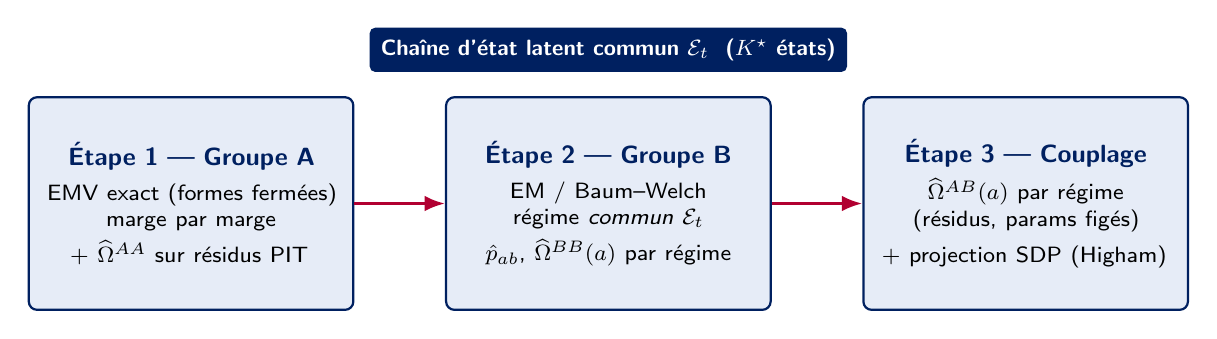
\begin{tikzpicture}[
  font=\sffamily\small,
  box/.style={rectangle, rounded corners=3pt, draw=nxnavy, line width=0.8pt,
              fill=nxlightblue, text width=3.7cm, align=center, inner sep=6pt, minimum height=2.7cm},
  lab/.style={rectangle, rounded corners=2pt, fill=nxnavy, text=white, inner sep=4pt, font=\sffamily\footnotesize\bfseries},
  arr/.style={-{Latex[length=2.6mm,width=2.0mm]}, line width=1.1pt, draw=nxred}]
\node[box] (a) {\textbf{\textcolor{nxnavy}{Étape 1 --- Groupe A}}\\[3pt]\footnotesize EMV exact (formes fermées)\\ marge par marge\\[2pt] $+\ \widehat\Omega^{AA}$ sur résidus PIT};
\node[box, right=1.15cm of a] (b) {\textbf{\textcolor{nxnavy}{Étape 2 --- Groupe B}}\\[3pt]\footnotesize EM / Baum--Welch\\ régime \emph{commun} $\Ecal_t$\\[2pt] $\hat p_{ab}$,\ $\widehat\Omega^{BB}(a)$ par régime};
\node[box, right=1.15cm of b] (c) {\textbf{\textcolor{nxnavy}{Étape 3 --- Couplage}}\\[3pt]\footnotesize $\widehat\Omega^{AB}(a)$ par régime\\ (résidus, params figés)\\[2pt] $+$ projection SDP (Higham)};
\node[lab, above=3mm of b] (top) {Chaîne d'état latent commun $\Ecal_t$ \ ($K^\star$ états)};
\draw[arr] (a) -- (b);
\draw[arr] (b) -- (c);
\end{tikzpicture}
\caption{Cascade d'estimation séquentielle (IFM). Chaque étape admet des mises à jour en \emph{forme fermée} (\S\ref{sec:closed}) ; seule l'Étape~2 itère (EM à ascension monotone).}
\label{fig:cascade}
\end{figure}

\subsubsection{Étape 1 --- Groupe A : EMV exact + corrélations sur résidus}
Pour chaque $i\in A$, maximiser la vraisemblance conditionnelle exacte (Prop.~\ref{prop:mle1}), puis calculer les résidus PIT et $\widehat\Omega^{AA}=\widehat\Corr(\widehat\eps^{A})$. La consistance des marges est garantie indépendamment de la dépendance croisée (estimateur IFM), au prix d'une perte d'efficience \emph{modérée et quantifiable}, largement compensée par le gain de conditionnement.

\subsubsection{Étape 2 --- Groupe B : EM (filtre de Hamilton) à régime commun}
Les facteurs du Groupe~B étant couplés par le régime \emph{commun}, ils s'estiment \emph{conjointement} par l'algorithme EM / Baum--Welch : une étape~E (filtre de Hamilton vers l'avant $+$ lisseur de Kim vers l'arrière) calcule les probabilités lissées $\hat\xi_t(a)=\Prob(\Ecal_t=a\mid\Xcal_n)$ et de transition $\hat\xi_t(a,b)$ ; une étape~M met à jour, \emph{en forme fermée} (\S\ref{sec:closed}), les paramètres et corrélations par régime. L'EM garantit l'ascension \emph{monotone} de la vraisemblance et gère proprement l'intégration de l'état latent : plus \emph{rapide} et plus \emph{robuste} que la maximisation directe (sous réserve de planchers de variance).

\subsubsection{Étape 3 --- corrélations inter-groupes par régime}
On \emph{fige} les paramètres des Étapes~1--2 et les probabilités lissées. Les seules inconnues restantes sont les corrélations croisées $\Omega^{AB}(a)$ (par régime). À marges fixées, la maximisation de la log-vraisemblance globale de la copule gaussienne se réduit à la corrélation pondérée des résidus (forme fermée, \S\ref{sec:closed}). On assemble la matrice par régime et on la projette sur le cône SDP le plus proche (Higham, 1988/2002), \emph{régime par régime}, condition de la décomposition de Cholesky :
\[
\Omega(a)=\begin{pmatrix}\Omega^{AA} & \Omega^{AB}(a)\\[2pt] \Omega^{AB}(a)\transp & \Omega^{BB}(a)\end{pmatrix}
\ \xrightarrow{\ \text{Higham}\ }\ \Omega^{\mathrm{SDP}}(a).
\]

\subsection{Formes fermées des estimateurs}
\label{sec:closed}

C'est le point que la présente version développe : \emph{partout où une forme fermée existe, on la donne}. Trois familles d'estimateurs sont concernées, récapitulées en Table~\ref{tab:closed}.

\paragraph{(A) Facteurs gaussiens à discrétisation exacte --- EMV conditionnel $=$ moindres carrés.}
La discrétisation exacte d'un Ornstein--Uhlenbeck donne un AR(1) \emph{gaussien} : la vraisemblance conditionnelle est gaussienne, son maximum est l'estimateur des moindres carrés ordinaires (MCO), \emph{en forme fermée}, suivi d'une inversion analytique des paramètres structurels. Pour un facteur scalaire $y_{t+h}=\beta y_t+c+\xi_{t+h}$ (Black--Karasinski sur $y=\ln s$ ; ou un OU) :

\begin{definitionbox}
\[
\hat\beta=\frac{\sum_t (y_t-\bar y_-)(y_{t+h}-\bar y_+)}{\sum_t (y_t-\bar y_-)^2},\quad
\hat c=\bar y_+-\hat\beta\,\bar y_-,\quad
\hat v=\frac{1}{n-1}\sum_t \widehat\xi_{t+h}^{\,2},
\]
puis l'inversion des paramètres structurels, en forme fermée,
\[
\hat k=-\frac{\ln\hat\beta}{h},\qquad
\hat\theta=\frac{\hat c}{1-\hat\beta},\qquad
\hat\sigma=\sqrt{\;\hat v\,\frac{-2\ln\hat\beta}{h\,(1-\hat\beta^{2})}\;}\,,
\]
où $\bar y_-,\bar y_+$ sont les moyennes empiriques de $(y_t)$ et $(y_{t+h})$.
\end{definitionbox}

\noindent Pour le \textbf{V2F} (structure triangulaire : le facteur court revient vers le facteur long), la même logique s'applique en cascade. Le facteur \emph{long} est un OU autonome estimé par le bloc ci-dessus, donnant $(\hat\kappa_2,\hat\mu,\hat\sigma_2)$. Le facteur \emph{court} se régresse alors, en forme fermée, sur $(q^s_t,q^l_t)$ :

\begin{definitionbox}
\[
\hat\beta_s=\frac{\sum_t (q^s_t-q^l_t)\,(q^s_{t+h}-q^l_t)}{\sum_t (q^s_t-q^l_t)^2},\qquad
\hat\kappa_1=-\frac{\ln\hat\beta_s}{h},\qquad
\hat\sigma_1=\sqrt{\;\hat v_s\,\frac{-2\ln\hat\beta_s}{h\,(1-\hat\beta_s^{2})}\;},
\]
et, si $\rho\neq 0$, $\ \hat\rho=\widehat\Corr(\widehat\xi^{\,s},\widehat\xi^{\,l})$ (corrélation des résidus des deux régressions).
\end{definitionbox}

\noindent \emph{Cette cascade de régressions coïncide avec la « double régression linéaire » de la revue, mais elle n'est pas une simple initialisation : c'est l'EMV conditionnel exact, donc l'estimateur \textbf{efficient}}, et c'est précisément ce qui justifie de la préférer aux cibles distributionnelles. (De façon équivalente, on estime le VAR(1) gaussien sans contrainte par MCO multivarié $\widehat\Phi$, puis $A=-h^{-1}\log\widehat\Phi$ donne les $\kappa_i$ par ses valeurs propres et l'équation de Lyapunov discrète $\widehat V=\Sigma_\infty-\widehat\Phi\,\Sigma_\infty\widehat\Phi\transp$ fournit $\Sigma_w$, donc $\sigma_1,\sigma_2,\rho$.)

\paragraph{(B) Hardy RSLN --- pas d'EMV en forme fermée, mais une itération EM entièrement explicite.}
L'\emph{étape E} est une récurrence fermée : filtre de Hamilton vers l'avant
\[
\xi_{t\mid t-1}(a)=\sum_b \xi_{t-1\mid t-1}(b)\,p_{ba},\qquad
\xi_{t\mid t}(a)=\frac{\xi_{t\mid t-1}(a)\,f_a(x_t)}{\sum_{a'}\xi_{t\mid t-1}(a')\,f_{a'}(x_t)},
\]
($f_a$ : densité $\Ncal(\mu_a,\sigma_a^2)$ du log-rendement en régime $a$), puis lisseur de Kim vers l'arrière donnant $\hat\xi_t(a)$ et $\hat\xi_t(a,b)$. L'\emph{étape M} admet des mises à jour \emph{en forme fermée} :

\begin{definitionbox}
\[
\hat\mu_a=\frac{\sum_t \hat\xi_t(a)\,x_t}{\sum_t \hat\xi_t(a)},\qquad
\hat\sigma_a^{2}=\frac{\sum_t \hat\xi_t(a)\,(x_t-\hat\mu_a)^2}{\sum_t \hat\xi_t(a)},\qquad
\hat p_{ab}=\frac{\sum_t \hat\xi_t(a,b)}{\sum_t \hat\xi_t(a)}.
\]
\end{definitionbox}

\noindent Pour le Groupe~B \emph{joint} (plusieurs actifs partageant $\Ecal_t$), $\hat\mu_a$ et $\hat\sigma^2_a$ deviennent un vecteur-moyenne et une matrice de covariance pondérés, dont on déduit $\widehat\Omega^{BB}(a)$. Chaque itération EM est donc fermée ; seule la boucle externe itère, avec ascension monotone garantie.

\paragraph{(C) Corrélations croisées par régime --- forme fermée.}
À marges figées, la log-vraisemblance de la copule gaussienne est concave en la corrélation et son maximum est la corrélation empirique (pondérée par les responsabilités de régime) des résidus standardisés :

\begin{definitionbox}
\[
\widehat\Omega^{AB}(a)=\frac{\sum_t \hat\xi_t(a)\,\widehat\eps^{A}_t\,(\widehat\eps^{B}_t)\transp}{\sum_t \hat\xi_t(a)}\,,
\qquad
\widehat\Omega^{AA}=\widehat\Corr(\widehat\eps^{A}),\quad
\widehat\Omega^{BB}(a)=\frac{\sum_t \hat\xi_t(a)\,\widehat\eps^{B}_t\,(\widehat\eps^{B}_t)\transp}{\sum_t \hat\xi_t(a)}.
\]
\end{definitionbox}

\paragraph{(D) CIR --- forme fermée pour l'initialisation seulement.}
La loi de transition exacte étant un $\chi^2$ décentré, l'EMV n'a \emph{pas} de forme fermée (optimisation numérique). En revanche, l'initialisation par schéma d'Euler est fermée : la régression sans constante
\[
\frac{s_{t+h}-s_t}{\sqrt{|s_t|}}\ \sim\ c_1\,\frac{1}{\sqrt{|s_t|}}+c_2\,\sqrt{|s_t|}+\eps_t
\quad\Longrightarrow\quad
\hat\kappa=-\frac{\hat c_2}{h},\ \ \hat\theta=\frac{\hat c_1}{\hat\kappa\,h},\ \ \hat\sigma^2=\frac{\widehat\Var(\eps)}{h},
\]
fournit un point de départ ; le résidu PIT du CIR s'obtient ensuite via la fonction de répartition du $\chi^2$ décentré (fonction spéciale, sans inversion itérative au-delà de son évaluation).

\begin{table}[h]
\centering\small
\renewcommand{\arraystretch}{1.3}
\begin{tabularx}{\textwidth}{@{}l c X@{}}
\toprule
\textbf{Facteur / quantité} & \textbf{Forme fermée ?} & \textbf{Estimateur} \\
\midrule
V2F (infl., taux réels) & Oui ($=$ EMV exact) & Cascade MCO $+$ inversion analytique $(\kappa_i,\sigma_i,\mu,\rho)$ \\
Black--Karasinski (dette priv.) & Oui ($=$ EMV exact) & MCO scalaire $+$ inversion $(k,\theta,\sigma)$ \\
BS \emph{unsmoothing} (PE/immo/infra) & Oui & Moyenne/variance des log-rendements déslissés \\
Hardy RSLN (actions) & Oui \emph{par itération} EM & Étape M pondérée fermée $+$ E-step récursif \\
CIR (crédit IG) & Init.\ oui, EMV non & MCO d'Euler (init) $+$ EMV $\chi^2$ décentré numérique \\
$\Omega^{AA},\ \Omega^{BB}(a),\ \Omega^{AB}(a)$ & Oui & Corrélation (pondérée) des résidus PIT \\
\bottomrule
\end{tabularx}
\caption{Disponibilité des formes fermées dans le cadre proposé. Cinq des six lignes admettent une forme fermée (exacte ou par itération EM) ; seul l'EMV du CIR requiert une optimisation, initialisée en forme fermée.}
\label{tab:closed}
\end{table}

\subsection{Choix du nombre d'états $K^\star$}
\label{sec:K}

Le nombre d'états est sélectionné par une analyse de la vraisemblance optimale par cardinalité. On ajuste pour $K=1,2,3,\dots$ et on relève $\ell^\star(K)$. Les modèles étant emboîtés, $\ell^\star$ croît avec $K$ ; on retient $K^\star$ par critère d'information
\[
\mathrm{BIC}(K)=-2\,\ell^\star(K)+p_K\,\ln n\qquad(\text{ou AIC}),
\]
de façon équivalente par la \emph{méthode du coude} sur la courbe $\ell^\star(K)$. Le test du rapport de vraisemblance pour le \emph{nombre} de régimes est \emph{non standard} (paramètres de nuisance non identifiés sous l'hypothèse nulle, score dégénéré --- Hansen, 1992 ; Garcia, 1998 ; Cho \& White, 2007) : le critère d'information / le coude est donc le choix pragmatique et défendable. Un \emph{unique} régime à $K^\star$ états remplace les $k$ chaînes séparées à deux états : il définit le régime de marché \emph{une seule fois} (plus d'intersections vides) et \emph{résout l'explosion combinatoire} en optimisant la cardinalité « au strict nécessaire » (de $2^k$ à $K^\star$).

\subsection{Simulation unifiée et cohérente}

La calibration achevée, la simulation utilise \emph{directement} la représentation globale.

\begin{enumerate}
\item \textbf{Régime.} Tirer le chemin \emph{unique} $\{\Ecal_t\}$ selon $P$ --- l'artifice de l'uniforme commune disparaît, le co-mouvement des régimes est \emph{intrinsèque}.
\item \textbf{Chocs corrélés par régime.} À chaque pas, $\eps_{t+h}=L(\Ecal_t)\,z_{t+h}$ avec $z_{t+h}\sim\Ncal(0,I)$ et $L(a)L(a)\transp=\Omega^{\mathrm{SDP}}(a)$ : les browniens sont déduits des corrélations \emph{par régime}, couplant correctement Groupes~A et~B.
\item \textbf{Propagation.} Évaluer chaque facteur par sa récurrence AR avec les coefficients du régime courant (constants pour le Groupe~A), les facteurs non gaussiens (CIR) étant restitués par l'étape inverse-PIT / Alfonsi de sorte que le score normal pilote la bonne marge.
\end{enumerate}

\begin{mabox}[Propriétés du dispositif proposé]
\textbf{Cohérence estimation/simulation} : une \emph{seule} loi (copule gaussienne par régime) sous-tend les deux phases. \textbf{Régimes systémiques} : la chaîne commune reproduit l'entrée \emph{conjointe} des actifs risqués en stress, donc la dépendance de queue. \textbf{Corrélations de stress bien définies} : conditionnellement à $\Ecal_t=a$, sur plein support --- ni intersection vide, ni biais de sélection. \textbf{Parcimonie} : $K^\star$ optimal contre l'explosion $2^k$. \textbf{Robustesse et formes fermées} : EMV/EM conditionnels (consistants en forte persistance), estimateurs explicites là où ils existent, corrélations sur résidus stationnaires.
\end{mabox}

\section{Synthèse comparative}

La Table~\ref{tab:synth} récapitule, point critiqué par point critiqué, la conséquence et le correctif proposé dans le cadre unifié.

\begin{table}[h]
\centering\small
\renewcommand{\arraystretch}{1.4}
\setlength{\tabcolsep}{5pt}
\begin{tabularx}{\textwidth}{>{\raggedright\arraybackslash}p{3.5cm}|X|X}
\toprule
\textbf{Point critiqué} & \textbf{Conséquence} & \textbf{Correctif proposé} \\
\midrule
\rowcolor{nxlightblue} Cibles distributionnelles (MM/GMM) &
Forte variance, mauvais conditionnement ($\sigma^2/\kappa$), instabilité à la fenêtre ; perte d'efficience &
EMV conditionnel exact (densité déjà disponible) en \emph{forme fermée} ; pondération efficiente ; $J$-test \\
\rowcolor{nxoffwhite} Initialisation hors régime stationnaire &
Trajectoire transitoire : moyenne et dispersion empiriques \emph{ne convergent pas} vers les cibles stationnaires $\Rightarrow$ biais ($\hat\kappa\!\downarrow$, $\hat\sigma\!\uparrow$) ; correction $\widehat\Omega^2$ circulaire (admis dans la revue) &
EMV conditionnel (valide en local-de-l'unité) ; travail sur résidus standardisés ; tests ADF/PP/KPSS en niveau \\
\rowcolor{nxlightblue} Corrélations / dispersions de niveau &
Co-tendance des niveaux $\Rightarrow$ quantités gonflées (régression fallacieuse) ; Higham régularise un biais &
Corrélations sur résidus PIT, bruit blanc stationnaire \\
\rowcolor{nxoffwhite} Hardy : vraisemblance brute &
Vraisemblance non bornée, maxima fallacieux, échange d'étiquettes &
EM/Baum--Welch à ascension monotone (étape M fermée) ; planchers de variance \\
\rowcolor{nxlightblue} Corrélations par intersection de stress &
Intersections vides/exiguës ($\sim 0{,}26^k$), régime incohérent, non-SDP &
Régime \emph{commun} $\Ecal_t$ ; corrélations par régime sur plein support \\
\rowcolor{nxoffwhite} Calibrage séparé des chaînes &
Pas de facteur latent commun ; explosion $2^k$ ; queue sous-estimée &
MS-VAR à régime latent partagé, $K^\star$ optimal (BIC/coude) \\
\rowcolor{nxlightblue} Simulation par uniforme commune &
Dépendance comonotone non estimée, dépendante de l'étiquetage, incohérente &
Simulation directe : un seul régime, chocs $L(\Ecal_t)z$ par régime \\
\bottomrule
\end{tabularx}
\caption{Synthèse des trois critiques et du cadre unifié proposé.}
\label{tab:synth}
\end{table}

\section{Conclusion}

Le GSE du régime repose sur des choix de modélisation solides ; les fragilités identifiées portent sur l'\emph{estimation} et le \emph{couplage}, non sur les EDS retenues. Le fil conducteur des trois critiques est unique : un \emph{décalage entre la quantité visée et la quantité estimée}. Les cibles distributionnelles visent des moments \emph{stationnaires} mais sont appariées à des statistiques calculées sur une trajectoire \emph{transitoire} partant de conditions initiales figées --- d'où un biais directionnel ($\hat\kappa$ trop faible, $\hat\sigma$ trop fort) que la revue observe sans le nommer, et une circularité qu'elle admet. Le modèle de Hardy est estimé chaîne par chaîne puis recollé par des procédés (intersections de stress, uniforme commune) qui n'ont pas de fondement probabiliste unique et sous-estiment la dépendance de queue.

Le cadre proposé répond à ces trois points d'un seul tenant : une \emph{représentation autorégressive universelle} ramène chaque facteur à une récurrence dont les coefficients dépendent d'un \emph{régime latent commun} ; l'estimation procède par \emph{maximum de vraisemblance jointe et séquentielle}, avec des \emph{formes fermées} explicites pour cinq des six familles d'estimateurs ; la dépendance est portée par des \emph{résidus standardisés} (copule gaussienne cohérente avec la simulation) et par une \emph{chaîne d'état unique} dont la cardinalité est choisie de façon parcimonieuse. Il en résulte un dispositif où l'estimation et la simulation partagent une seule et même loi, où les corrélations de stress sont bien définies, et où la robustesse numérique est sensiblement accrue. Tout calibrage embarque une erreur d'estimation ; le choix final des méthodes et paramètres relève de l'IRCANTEC.

\newpage
\phantomsection
\addcontentsline{toc}{section}{Références}
{\noindent\sffamily\Large\bfseries\color{nxnavy}Références\par}
\vspace{4mm}
{\small
\begin{list}{}{\setlength{\leftmargin}{1.2em}\setlength{\itemindent}{-1.2em}\setlength{\itemsep}{2pt}}
\item Baum, L.\,E., Petrie, T., Soules, G., \& Weiss, N. (1970). A maximization technique occurring in the statistical analysis of probabilistic functions of Markov chains. \emph{Annals of Mathematical Statistics}, 41(1), 164--171.
\item Cho, J.\,S., \& White, H. (2007). Testing for regime switching. \emph{Econometrica}, 75(6), 1671--1720.
\item Dempster, A.\,P., Laird, N.\,M., \& Rubin, D.\,B. (1977). Maximum likelihood from incomplete data via the EM algorithm. \emph{Journal of the Royal Statistical Society B}, 39(1), 1--38.
\item Frühwirth-Schnatter, S. (2006). \emph{Finite Mixture and Markov Switching Models}. Springer.
\item Garcia, R. (1998). Asymptotic null distribution of the likelihood ratio test in Markov switching models. \emph{International Economic Review}, 39(3), 763--788.
\item Granger, C.\,W.\,J., \& Newbold, P. (1974). Spurious regressions in econometrics. \emph{Journal of Econometrics}, 2(2), 111--120.
\item Hamilton, J.\,D. (1989). A new approach to the economic analysis of nonstationary time series and the business cycle. \emph{Econometrica}, 57(2), 357--384.
\item Hansen, B.\,E. (1992). The likelihood ratio test under nonstandard conditions: testing the Markov switching model of GNP. \emph{Journal of Applied Econometrics}, 7(S1), S61--S82.
\item Hansen, L.\,P. (1982). Large sample properties of generalized method of moments estimators. \emph{Econometrica}, 50(4), 1029--1054.
\item Hartigan, J.\,A. (1985). A failure of likelihood asymptotics for normal mixtures. In \emph{Proceedings of the Berkeley Conference}, vol.~2, 807--810.
\item Higham, N.\,J. (2002). Computing the nearest correlation matrix --- a problem from finance. \emph{IMA Journal of Numerical Analysis}, 22(3), 329--343.
\item Joe, H., \& Xu, J.\,J. (1996). \emph{The estimation method of inference functions for margins for multivariate models}. Technical Report 166, University of British Columbia.
\item Kim, C.-J. (1994). Dynamic linear models with Markov-switching. \emph{Journal of Econometrics}, 60(1--2), 1--22.
\item Kim, C.-J., \& Nelson, C.\,R. (1999). \emph{State-Space Models with Regime Switching}. MIT Press.
\item Krolzig, H.-M. (1997). \emph{Markov-Switching Vector Autoregressions}. Springer.
\item Kwiatkowski, D., Phillips, P.\,C.\,B., Schmidt, P., \& Shin, Y. (1992). Testing the null hypothesis of stationarity against the alternative of a unit root. \emph{Journal of Econometrics}, 54(1--3), 159--178.
\item Phillips, P.\,C.\,B. (1986). Understanding spurious regressions in econometrics. \emph{Journal of Econometrics}, 33(3), 311--340.
\end{list}
}

\vspace{6mm}
\noindent{\footnotesize\color{nxgray}\rule{\textwidth}{0.3pt}\\[3pt]
Note critique méthodologique complémentaire à la revue du GSE. Document confidentiel. Les expressions et procédures présentées décrivent une approche alternative ; tout calibrage embarque une erreur d'estimation, et le choix final des méthodes et paramètres relève de l'IRCANTEC.}

\end{document}